%!TEX root = ./slopecd.tex
\section{Introduction}\label{sec:introduction}
%%%%%%%%%%%%%%%%%%%%%%%%%%%%%%%%%%%%%%%%%%%%%%

In this paper we present a novel numerical algorithm for Sorted L-One Penalized
Estimation (SLOPE)~\cite{bogdan2013, bogdan2015}, defined as
\begin{equation}
  \label{eq:slope-problem}
  \operatorname{minimize}_{\beta \in \mathbb{R}^p}
  P(\beta) = L(\beta) + J(\beta)
\end{equation}
where we take \(L\) to be smooth and twice differentiable and
\begin{equation}
  \label{eq:sorted-l1-norm}
  J(\beta) = \sum_{j=1}^p \lambda_j|\beta_{(j; \beta)}|
\end{equation}
is the \emph{sorted \(\ell_1\) norm}, defined such that
\[
  |\beta_{(1; \beta)}| \geq |\beta_{(2; \beta)}| \geq \cdots \geq |\beta_{(p; \beta)}|,
\]
and \(\lambda\) is a fixed non-increasing and non-negative
sequence.\footnote{In most works on SLOPE, the permutation operator is written
as \((i)\). But for reasons that will eventually become clear, we instead write
\((i; \beta)\) to make the dependence on \(\beta\) explicit.}

SLOPE is a sparse regression \mm{can be used for classif too. For me slope is the penalty, and so the 1st sentence could be rewritten too} method that has become increasingly popular due to
several appealing properties, such as its ability to control false discovery
rate~\cite{bogdan2015, kos2020}, cluster coefficients~\cite{figueiredo2016,
schneider2020a}, and recover sparsity and ordering patterns in the
solution~\cite{bogdan2022}. Unlike other competing sparse regularization methods such
as MCP~\cite{zhang2010} and SCAD~\cite{fan2001}, SLOPE is also a convex
problem~\cite{bogdan2015}.

In spite of the availability of predictor screening rules~\cite{elvira2022,
larsson2020c}, which help speed up SLOPE in the high-dimensional regime,
current state-of-the-art algorithms for SLOPE perform poorly in comparison to
those of other, more established, penalization methods such as the lasso
(\(\ell_1\)-norm regularization) and ridge regression (\(\ell_2\)-norm
regularization). As a small illustration of this issue, we compared the
speed at which the SLOPE and glmnet packages fit a complete regularization
path for the bcTCGA data set. SLOPE takes x seconds to fit the full path,
whilst glmnet requires only y seconds. \mm{Maybe this is too much detail for an introduction: if we want to be rigorous, we need to specify the path, the stopping criterion (it's hard to match what glmnet does exactly from my experience). I would be OK with just saying: solving SLOPE is not as fast as Lasso for now}

This lackluster performance has hampered the applicability of SLOPE to many
real-world applications, \mm{I would comment out the rest of the sentence: in the intro it's quite understandable that if an estimator is slow to compute people will not use it too much} particularly because users often need to solve SLOPE
repeatedly when tuning hyper-parameters, for instance in
cross-validation, or when fitting SLOPE as part of Adaptive Bayesian
SLOPE~\cite{jiang2022}.

A major reason for why algorithms for solving other regression models with
non-differentiable penalties,\mm{we have not mentioned non differentiability so far, it may confuse a bit the reader. I would just say ``for solving models with penalties such as the L1 norm, MCP... is that the separability of these penalties makes them amenable to coordiante descent algorithms. On the contrary, SLOPE is not separable and one must resort to FISTA or ADMM''} such as the lasso, MCP, and SCAD, enjoy better
performance is that they minimize their objectives using coordinate
descent~\cite{breheny2011, friedman2010} rather than proximal gradient descent
algorithms such as FISTA~\cite{beck2009} and the
alternating direction method of multipliers method (ADMM)~\cite{boyd2010},
which are both used in the current version of the SLOPE package.
\jl{Add benchopt reference.}
\mm{For which point exactly? I did not find a ref for your SLOPE R package, what's the good way to cite it? There also is PyOWL https://github.com/vene/pyowl}

Applying coordinate descent to SLOPE is, however, not quite straightforward
because convergence guarantees for coordinate descent require the
objective to be separable, which, as we can see from \eqref{eq:sorted-l1-norm}
is not the case for SLOPE.

% The resulting solution \(\hat{\beta}\) has the property that it can cluster the
% coefficients by their magnitudes, such that \(\mathcal{C}=
% \{j: |\beta_j|=c\}\) for some \(c\).

In this article we address this problem by introducing a new, highly effective
algorithm for SLOPE based on a hybrid proximal gradient and coordinate descent
scheme. Our method features convergence guarantees and reduces the time
required to fit SLOPE by orders of magnitude in our empirical experiments.

\begin{figure}[htbp]
  \centering
  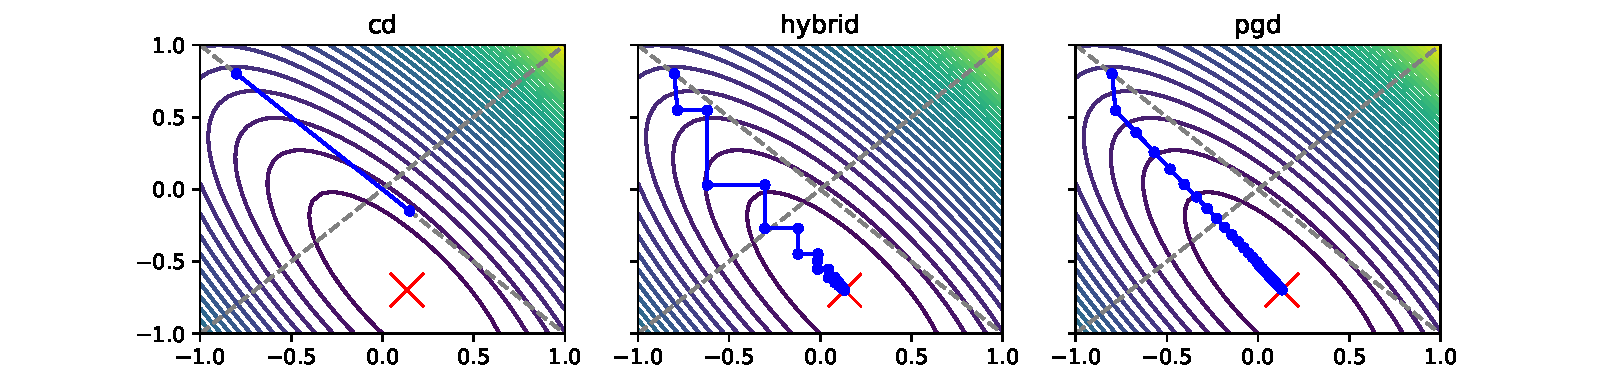
\includegraphics[scale=0.62]{illustration_solvers.pdf}
  \caption{Illustration of proposed solver.}
  \label{fig:illustration-solver}
\end{figure}
